\documentclass[]{article}
\usepackage{lmodern}
\usepackage{amssymb,amsmath}
\usepackage{ifxetex,ifluatex}
\usepackage{fixltx2e} % provides \textsubscript
\ifnum 0\ifxetex 1\fi\ifluatex 1\fi=0 % if pdftex
  \usepackage[T1]{fontenc}
  \usepackage[utf8]{inputenc}
\else % if luatex or xelatex
  \ifxetex
    \usepackage{mathspec}
  \else
    \usepackage{fontspec}
  \fi
  \defaultfontfeatures{Ligatures=TeX,Scale=MatchLowercase}
\fi
% use upquote if available, for straight quotes in verbatim environments
\IfFileExists{upquote.sty}{\usepackage{upquote}}{}
% use microtype if available
\IfFileExists{microtype.sty}{%
\usepackage{microtype}
\UseMicrotypeSet[protrusion]{basicmath} % disable protrusion for tt fonts
}{}
\usepackage[margin=1in]{geometry}
\usepackage{hyperref}
\hypersetup{unicode=true,
            pdftitle={Zajęcia z R},
            pdfborder={0 0 0},
            breaklinks=true}
\urlstyle{same}  % don't use monospace font for urls
\usepackage{graphicx,grffile}
\makeatletter
\def\maxwidth{\ifdim\Gin@nat@width>\linewidth\linewidth\else\Gin@nat@width\fi}
\def\maxheight{\ifdim\Gin@nat@height>\textheight\textheight\else\Gin@nat@height\fi}
\makeatother
% Scale images if necessary, so that they will not overflow the page
% margins by default, and it is still possible to overwrite the defaults
% using explicit options in \includegraphics[width, height, ...]{}
\setkeys{Gin}{width=\maxwidth,height=\maxheight,keepaspectratio}
\IfFileExists{parskip.sty}{%
\usepackage{parskip}
}{% else
\setlength{\parindent}{0pt}
\setlength{\parskip}{6pt plus 2pt minus 1pt}
}
\setlength{\emergencystretch}{3em}  % prevent overfull lines
\providecommand{\tightlist}{%
  \setlength{\itemsep}{0pt}\setlength{\parskip}{0pt}}
\setcounter{secnumdepth}{0}
% Redefines (sub)paragraphs to behave more like sections
\ifx\paragraph\undefined\else
\let\oldparagraph\paragraph
\renewcommand{\paragraph}[1]{\oldparagraph{#1}\mbox{}}
\fi
\ifx\subparagraph\undefined\else
\let\oldsubparagraph\subparagraph
\renewcommand{\subparagraph}[1]{\oldsubparagraph{#1}\mbox{}}
\fi

%%% Use protect on footnotes to avoid problems with footnotes in titles
\let\rmarkdownfootnote\footnote%
\def\footnote{\protect\rmarkdownfootnote}

%%% Change title format to be more compact
\usepackage{titling}

% Create subtitle command for use in maketitle
\providecommand{\subtitle}[1]{
  \posttitle{
    \begin{center}\large#1\end{center}
    }
}

\setlength{\droptitle}{-2em}

  \title{Zajęcia z R}
    \pretitle{\vspace{\droptitle}\centering\huge}
  \posttitle{\par}
    \author{}
    \preauthor{}\postauthor{}
    \date{}
    \predate{}\postdate{}
  

\begin{document}
\maketitle

\subsection{Wprowadzenie}\label{wprowadzenie}

\textbf{R} -- język programowania; środowisko do obliczeń statystycznych
i wizualizacji (nie tylko). Oprogramowanie R jest projektem GNU opartym
o licencję GNU GPL, jest więc zupełnie darmowy zarówno do zastosowań
edukacyjnych jak i biznesowych.

\textbf{Rstudio} - najpopularniejszy edytor do języka R.

Instalacja i inne bardzo przydatne informacje można znaleźć w wielu
tutorialach dostępnych online. Np. Przemysław Biecek
\href{http://biecek.pl/r/przewodnikpopakiecierwydanieiiiinternet.pdf}{Przewodnik
po pakiecie R}.

RStudio składa się z kilku podokien i narzędzi:

\begin{itemize}
\item
  Konsola (\emph{Console}) -- tutaj możesz wpisywać bezpośrednio kod,
\item
  Okno środowiska (\emph{Environment}) -- wyświetlane tu są wszystkie
  zapisane w pamięci zmienne, jak i funkcje. Środowisko można zapisać,
  jak również wczytać. Używając tego okna można również importować dane
  z zewnątrz oraz przejrzeć historię wpisywanych linii kodu.
\item
  Okno z zakładkami -- tutaj możemy przeglądać strukturę plików na dysku
  (\emph{Files}), wyświetlać wykresy (\emph{Plots}), przeglądać
  zainstalowane pakietu (\emph{Packages}), szukać pomocy na temat
  funkcji z pakietów (\emph{Help}).
\item
  W R najczęściej chcemy pisać skrypty składające się z wielu linii,
  które następnie będziemy wykonywać. Do otwarcia nowego skryptu służy
  ikona Add R Script lub kombinacja klawiszy Ctrl+Shift+N.
\end{itemize}

\begin{figure}
\centering
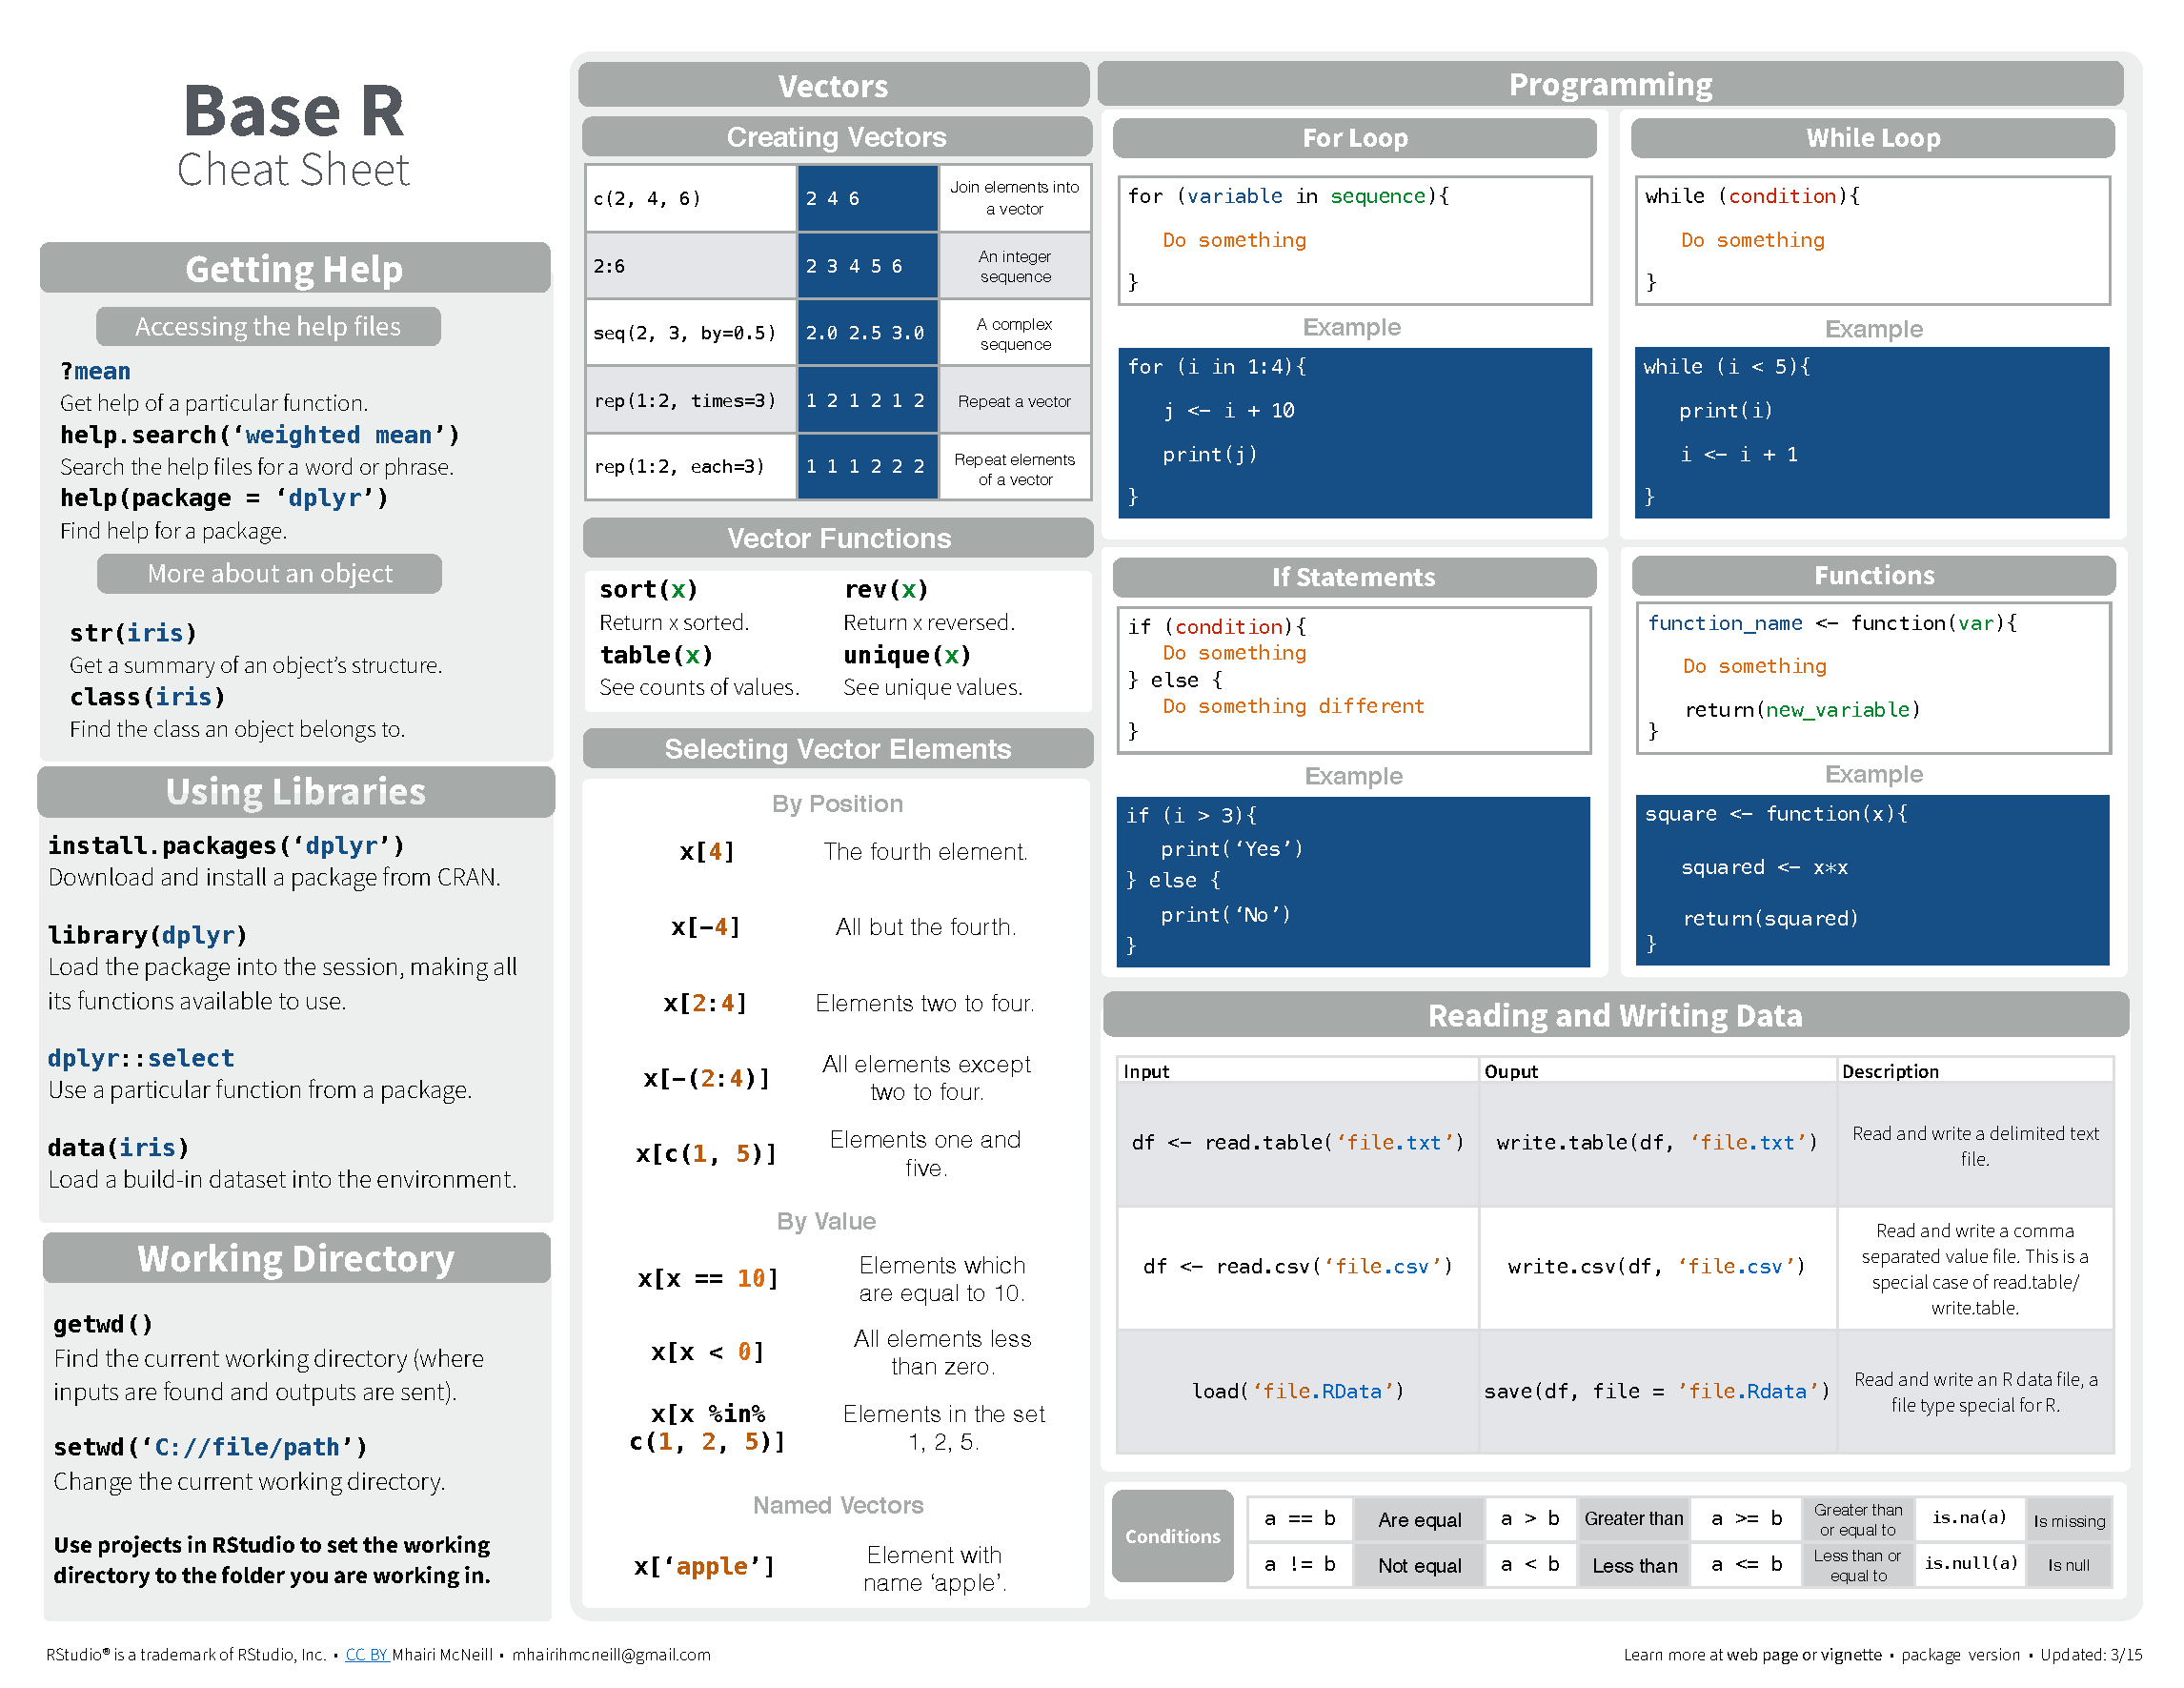
\includegraphics{base-r.pdf}
\caption{Podstawy R - cheat sheet}
\end{figure}

Funkcje -- zazwyczaj skonstruowane w sposób:

nazwa\_funkcji(x, y, \ldots{})

\begin{itemize}
\tightlist
\item
  x -- dane wejściowe
\item
  y -- dalsze argumenty, które mogą być Na przykład w funkcji
  \href{https://stat.ethz.ch/R-manual/R-devel/library/utils/html/read.table.html}{\texttt{read.csv()}},
  która służy do wczytywania danych w formacie csv:
\end{itemize}

\texttt{read.csv(file,\ header\ =\ TRUE,\ sep\ =\ ",",\ quote\ =\ "\textbackslash{}"",\ dec\ =\ ".",\ fill\ =\ TRUE,\ comment.char\ =\ "",\ ...)}

Wynik działania danej funkcji możemy przypisać do zmiennej:
\texttt{dane\ =\ read.csv(\ldots{})}

Typy obiektów w R:

\begin{itemize}
\tightlist
\item
  Wektory
\item
  Tekst
\item
  Macierze
\item
  Listy
\item
  Ramki danych (\textbf{data frames})
\end{itemize}

\emph{Wektory} - to najprostszy rodzaj struktury danych w R.

\texttt{wektor\ =\ c(10,\ 12,\ 16,\ -4,\ 3,\ 17,\ -1,\ 5,\ 12,\ 4)}

\emph{Ramki danych} Wczytywanie bazy danych - najczęściej w formacie
.csv \textgreater{} obiekt typu data frame Po wczytaniu danych warto
sprawdzić czy wszystko z nimi w porządku, np. uzywając str() lub
summary()

\texttt{str(dane)} \texttt{summary(dane)}

Po wywołaniu fukncji str() zobaczymy strukturę każdej z kolumn.
Pamiętaj, że aby przeprowadzac dalsze przetowrzenia na liczbach
odpowiednie kolumny muszą mięć odpowiednie formaty liczbowe - czyli
\textbf{int} lub \textbf{num} Dostęp do poszczególne kolumn - możemy
użyć znaku \$ czyli:

\texttt{dane\$nachylenie}

lub kwadratowcyh nawiasów:

\texttt{dane{[},4{]}}

Aby wywołac jakąś konkretną wartość z data frame możemy wpisać:

\texttt{dane{[}9,17{]}} gdzie w tym przypadku 9 to numer rzędu a 17
kolumny

\begin{center}\rule{0.5\linewidth}{\linethickness}\end{center}

Pakiety -- instalacja i wczytywanie W R dostępnych jest wiele funkcji
„bazowych'', jedną z nich jest \texttt{read.csv()}. Istenieje jednak
wiele dodatkowych pakietów zawierających fukkcje bardziej złożone i
służące określonym zadaniom. Aby wykorzystać funkcje z jakiegoś pakietu
należy najpierw go zainstalować (raz), następnie wczytać (każdorazowo
przy nowym projekcie). Służą do tego funkcje:

\texttt{install.packages(„nazwa\_pakietu”)}

\texttt{library(nazwa\_pakietu)}

Instalować pakiety można również wchodząc w zakładkę Packages.

Pomoc na temat danej funkcji możemy uzyskac wpisując:

\texttt{?nazwa\_funkcji}

\begin{center}\rule{0.5\linewidth}{\linethickness}\end{center}

\subsection{Analizy statystyczne w R}\label{analizy-statystyczne-w-r}

\begin{itemize}
\tightlist
\item
  Korelacja
\item
  Regresja, modele regresji
\item
  Prosta regresja liniowa
\item
  Regresja wieloraka
\end{itemize}

\textbf{Przed przystąpieniem do analiz warto sprawdzic poprawność
wczytanych danych oraz uzupełnić/usunąć wartości puste (\emph{NA})}

\subsubsection{Statystyki opisowe}\label{statystyki-opisowe}

Statystyki takie jak średnia, minimum, odchylenie standardowe,
mediana\ldots{} dla danej zmienniej uzyskamy poprzez wpisanie:

\texttt{mean()}

\texttt{min()}

\texttt{std()}

\texttt{median()}

\textbf{Uwaga!} jeżeli w danych danych mamy wartości puste - w R
oznaczane jako \emph{NA} (\emph{Not Available}) wynikiem wyżej
wymienionych operacji również będzie NA. Aby policzyć statystyki dla
wartości, które nie są NA nalezy dodać argument \texttt{na.rm\ =\ TRUE}
np.:

\texttt{mean(dane\$TPI200,\ na.rm\ =\ TRUE)}

\subsubsection{Proste wykresy}\label{proste-wykresy}

Proste wykresy mozna tworzyć za pomocą funckji \texttt{plot()}

Spróbuj utworzyć wykres zależności wysokości (HL) od wieku drzew oraz
Site Indexu (SI) od wysokości n.p.m. 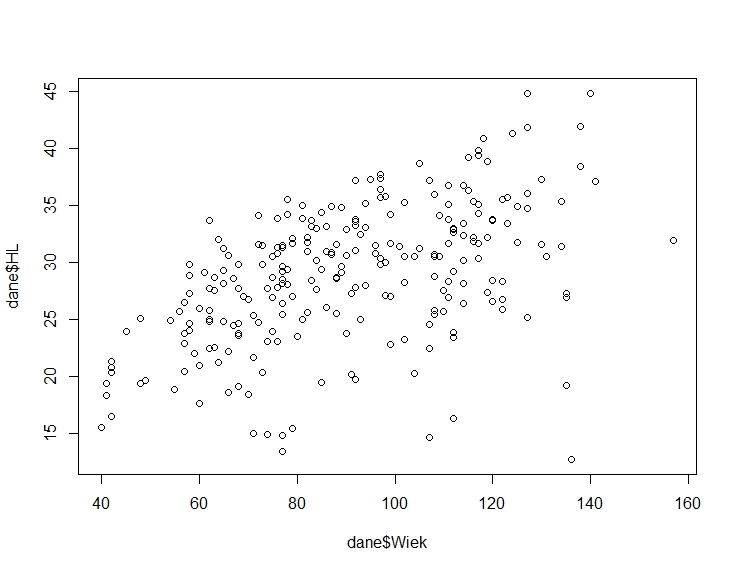
\includegraphics{plot1.jpeg}

Inne przydatne funkcje do wykresów to:

\begin{itemize}
\item
  Wykres rozrzutu z krzywą \texttt{scatter.smooth()}
\item
  Wykres ramka-wąsy \texttt{box.plot()}
\item
  Histogram \texttt{hist()}
\item
  Wykres gęstości \texttt{plot(density())}
\item
  Macierz wykresów rozrzutu \texttt{pairs()}
\end{itemize}

Wygeneruj kilka z wyżej wymienionych typów wykresów dla wybranych
zmiennych.

\subsubsection{Korelacja}\label{korelacja}

Do obliczenia korelacji między zmiennymi możemy użyć funkcji
\texttt{cor()}. Domyślnie mierzy ona korelacje Pearsona.

Wywołując pomoc dla funkcji \texttt{cor()} sprawdź jakie miary korelacji
są dostępne.

Korelację obliczymy tylko dla danych liczbowych - dlatego przed jej
obliczeniem wyodrębnimy cześć naszego data frame.

W tym celu wykorzystamy nawiasy kwadratowe.

Utwórz nowy obiekt \emph{dane\_subset}, który będzie zawierał kolumny 3,
4 i od 9 do 13, następnie oblicz macierz korelacji.

Macierz korelacji możemy zwizualizować za pomocą funkcji
\texttt{corrplot()} z pakietu \textbf{corrplot}

Zainstaluj i wczytaj powyższy pakiet a następnie zwizualizuj macierz
korelacji.

Do obliczenia istotności korelacji służy funkcja \texttt{cor.test()}

Ciekawe narzędzia do wizualizacji korelacji dostępne są w pakiecie
\texttt{corrplot}. Zanistaluj i wczytaj pakiet a następnie użyj funkcji
\texttt{corrplot()} do wizualizacji wcześniej obliczonej macierzy
korelacji.

\subsubsection{Regresja liniowa}\label{regresja-liniowa}

Do obliczenia modelu regresji liniowej służy funkcja \texttt{lm()}.
Formułę modelu podajemy w postaci:

Y \textasciitilde{} X1 + X2 + \ldots{}

Oblicz model regresji liniowej - jako zmienną objaśnianą wybierz
Wysokość a jako objaśniającą Wiek. Zapisz model jako obiekt
\emph{model1} i wywołaj go - pojawią się współczynniki a i b czyli
równanie regresji. Sprawdź inne parametry modelu poprzez zastosowanie
funkcji \texttt{summary()}

W podsumowaniu modelu znajdziemy między innymi wartość p (przedostatnia
kolumna) oraz współczynnik determinacji R2.

\subsubsection{Regresja nieliniowa}\label{regresja-nieliniowa}

Wykorzystamy zmienne wysokości NPM i SI w regresji wielomianowej
(\emph{polynomial}), która ma postać:

\texttt{lm(Y\ \textasciitilde{}\ poly(X,i))}, gdzie \emph{i} to stopień
wielomianu

Utwórz kilka modeli z różnym stopniem wielomianu i oszacuj, który z nich
jest najlepiej dopasowany.

\subsubsection{Predykcja na podstawie utworzonego
modelu}\label{predykcja-na-podstawie-utworzonego-modelu}

Funkcja \texttt{predict()} pozwala na obliczenie predykowanych wartości
na podstawie modelu regresji:

\texttt{predict(model,\ dane)}

\begin{center}\rule{0.5\linewidth}{\linethickness}\end{center}

\subsection{Wizualizacje w R}\label{wizualizacje-w-r}

Do bardziej zaawansowanych wizualizacji w R możemy wykorzystać pakiet
\texttt{ggplot2}

Zainstaluj i wczytaj pakiet \texttt{ggplot2}

Funkcja \texttt{ggplot} z tego pakietu charakteryzje się określoną
składnią, którą na bieżąco można ulepszać (tzn. dodawać coraz więcej
warstw, motwywów do już istniejącego wykresu). Spróbujmy stworzyć
``bazę'' pod nasz wykres:

\texttt{ggplot(dane,\ aes(x,y))}

aes - czyli \emph{aesthetics} określa które zmienne będą na osi X i osi
y

Stwórz bazę pod nasz wykres (na początku punktowy - \emph{scatterplot})
- wybierz zmienne NPM i SI.

Utworzony wykres, mimo iż wybraliśmy zmienne jest pusty. Aby coś się na
nim pojawiło należy sprecyzować czy wykres ma być punktowy, liniowy czy
innego rodzaju. Kolejne elementy, w tym określenie typu geometrii
wykresu będziemy dodawać używając znaku \textbf{+}

\texttt{ggplot(dane,\ aes(x,y))+\ \ \ \ \ geom\_point()}

Inne typy geometrii: \texttt{geom\_line()}, \texttt{geom\_smooth()},
\texttt{geom\_boxplot()} \ldots{}

Dodaj do istniejącego wykresu krzywą używając
\texttt{geom\_smooth(se\ =\ 0)}. Argument se pokazuje (lub w tym
przypadku nie) przedziały ufnośći.

Aby zmienić zakres osi x i y uzywamy odpowiednio (również używając znaku
+): \texttt{xlim(min,max)} i \texttt{ylim(min,max)}.

Tytuły wykresu i osi x i y: \texttt{labs(title\ =\ ,\ x\ =,\ y=\ )}

Kolory i kształty (argumenty \emph{color}, \emph{size}, \emph{fill})
możemy ustawić ``na stałe'' lub przypisać np. odmienne kolory lub
rozmiar w zależności od wartości jakiejś zmiennej, czyli:

\texttt{ggplot(dane,\ aes(x,y))+\ \ \ \ \ \ \ geom\_point(color\ =\ "red",\ size\ =\ 2)}

Jest to tzw. \emph{setting}, kolor czy kształt sa niezalezne od
zmiennych, definiujemy je poza \texttt{aes()}

\texttt{ggplot(dane,\ aes(x,y,\ color\ =\ a,\ size\ =\ b))+\ \ \ \ \ geom\_point()}

Jest to tzw. \emph{mapping}. Aby ustawić kolory zgodnie z
kategorią/zmienną argumenty \emph{color} i \emph{size} musza się zaleźć
wewnątrz \texttt{aes()}

\subsubsection{Wizualizacja wyników regresji liniowej i wielomianowej z
wykorzystaniem
ggplot}\label{wizualizacja-wynikow-regresji-liniowej-i-wielomianowej-z-wykorzystaniem-ggplot}

\begin{figure}
\centering
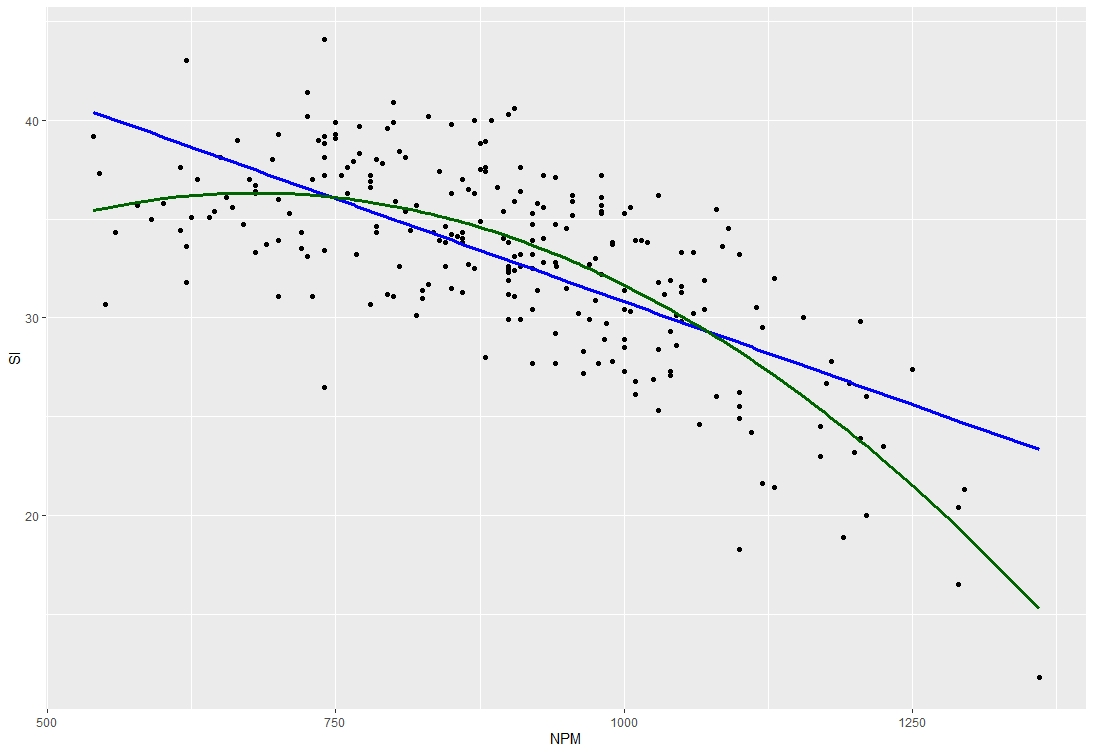
\includegraphics{REGRESJA.jpeg}
\caption{Porównanie regresji}
\end{figure}


\end{document}
